%-----------------------------------------------------------------------
%
%   UFRJ  - Universidade Federal do Rio de Janeiro
%   COPPE - Coordena��o dos Programas de P�s-gradua��o em Engenharia
%   PEE   - Programa de Engenharia El�trica
%
%   COE-835  Controle adaptativo
%
%   Relat�rio da simula��o
%                                                         Ramon R. Costa
%                                                         05/out/09, Rio
%-----------------------------------------------------------------------
\documentclass[11pt,a4paper]{article}
\usepackage[latin1]{inputenc} %pacote para utilizar palavras acentuadas
\usepackage{amsmath,amssymb}  %pacotes do AMS
\usepackage{latexsym}         %pacote para incluir s�mbolos (ex.\Box)
\usepackage{fancybox,fancyhdr}%pacote com frescuras
\usepackage{graphicx}         %pacote para incluir figuras tipo eps
\usepackage[portuguese]{babel}
\usepackage{xcolor}
\usepackage{float}
\usepackage[a4paper]{hyperref}% Make sure it comes last of your loaded packages
\hypersetup{
  verbose,
  plainpages=false,
  bookmarks=true,
  colorlinks=true,
  linkcolor=blue
}

%----------------------------------------------------------------------
%
%   Macros utilizados no LATEX
%                                                       Ramon R. Costa
%                                                       13/out/17, Rio
%----------------------------------------------------------------------
\newcount\m
\newcount\n

\def\twodigits#1{\ifnum #1<10 0\fi \number#1}

\def\hours{\n=\time \divide\n 60
    \m=-\n \multiply\m 60 \advance\m \time
    \twodigits\n:\twodigits\m}

\def\hora{\hours}

\def\fim{
  \medskip
  \begin{center}
    \rule[1mm]{30mm}{0.14mm}$\diamond$\rule[1mm]{30mm}{0.14mm}
  \end{center}
}

%----------------------------------------------------------------------
% A4 paper size & margins
\setlength {\textheight}    {25cm}%
\setlength {\textwidth}     {17.5cm}%
\setlength {\parindent}     {0mm}%
\setlength {\parskip}       {1mm}%
\setlength {\topmargin}     {-14mm}%
\setlength {\oddsidemargin} {-6mm}%
\setlength {\evensidemargin}{-6mm}%
\setlength {\columnsep}     {6mm}%

%----------------------------------------------------------------------
\def\codigo{COE-835}
\def\disciplina{Controle adaptativo}
\def\periodo{3o. período/2017}
\def\professor{Ramon}

\newcommand{\BOX}[1]{
  \framebox{{\color{magenta}\rule[-3mm]{1mm}{9mm}} ~~$\displaystyle
  \begin{aligned} #1 \end{aligned}$~~}\pagestyle{plain}
}

\newcommand{\RED}[1]{\colorbox{white}{\textcolor{red}{#1}}}
%\newcommand{\WoR}[1]{\colorbox{red}{\textcolor{white}{#1}}}
\newcommand{\BLU}[1]{\colorbox{white}{\textcolor{blue}{#1}}}
\newcommand{\GRE}[1]{\colorbox{green}{\textcolor{black}{#1}}}
\newcommand{\HI}[1]{\colorbox{yellow}{\textcolor{black}{#1}}}  %% Highlithed text

\newcommand{\estrela}[1]{
  \def\TXT{\RED{$\bigstar$ }}
  \hspace*{5mm}\TXT \hfill
  \parbox[t]{ \textwidth - \widthof{\TXT} - 5mm}{#1}
  \par
}

\def\Ltwo{\mbox{${\mathcal L}_2$}}
\def\Linf{\mbox{${\mathcal L}_\infty$}}

\newcommand{\sign}{\mbox{sign}}

\newcommand{\equacao}[2]{
  \makebox[40mm][l]{#1 \dotfill}: \quad \parbox[t]{8cm}
	{\begin{equation} \displaystyle
  \begin{aligned}
    #2
  \end{aligned} \end{equation}} \\
}

\newcommand{\sref}[1]{Section~\ref{#1}}
\newcommand{\fref}[1]{Fig.~\ref{#1}}
\newcommand{\tref}[1]{Table~\ref{#1}}
\newcommand{\thref}[1]{Theorem~\ref{#1}}
\newcommand{\aref}[1]{Assumption~\ref{#1}}
\newcommand{\norm}[1]{\left\lVert#1\right\rVert}
%\renewcommand{\qedsymbol}{}
\newcommand{\rev}[1]{{\color{red}#1}}
%\newcommand{\mat}[1]{\begin{bmatrix}#1\end{bmatrix}}

\newtheorem{remark}{Remark}
\newtheorem{lemma}{Lema}
\theoremstyle{plain}
\newtheorem{theorem}{Teorema}
%----------------------------------------------------------------------


\begin{document}
%---------------------------------------------------------------------
\pagestyle{fancy}%
\renewcommand{\headrulewidth}  {0.4pt}%
\renewcommand{\footrulewidth}  {0.4pt}%
\lhead{\bfseries{Relat�rio das simula��es}}%
\chead{}%
\rhead{\bfseries\thepage}%
\lfoot{}%
\cfoot{}%
\rfoot{[\hours] \quad \today}%
%---------------------------------------------------------------------
\begin{center}
  \huge{COE-835  Controle  adaptativo}  \\[20mm]

  \Large{Simula��es do exemplo 2} \\[20mm]
\end{center}


Algoritmo: \quad \HI{Gradiente normalizado}

\bigskip%
Caso: \quad \parbox[t]{10cm}{
  $~n = 1$ \quad (ordem da planta) \\[2mm]
  $n^* = 1$ \quad (grau relativo) \\[2mm]
  $n_p = 1$ \quad (\# de par�metros) \\[20mm]
}

%---------------------------------------------------------------------

\tableofcontents

\newpage%
%---------------------------------------------------------------------
\section{Resumo das equa��es do sistema simulado}

\equacao{Planta}
  {\dot{y}_p = a_p y_p + u}

\equacao{Modelo}
  {\dot{y}_m = -a_m y_m + r}

\equacao{Erro de sa�da}
  {e_0 = y_p - y_m}

\equacao{Lei de controle}
  {u = \theta y_p + r}

\equacao{Filtro}
  {\zeta = \frac{1}{s+a_m}\,y_p}

\equacao{Estimativa do erro}
  {\hat{e} = \frac{1}{s+a_m}\,[\theta y_p] - \theta\zeta}

\equacao{Erro de estimativa}
  {\varepsilon = e_0 - \hat{e}}

\equacao{Sinal normalizante}
  {m^2 = 1 + \zeta^2}

\equacao{Lei de adapta��o}
  {\dot{\theta} = - \frac{\gamma \varepsilon \zeta}{m^2}}


%---------------------------------------------------------------------
\section{Diagramas de blocos}

\begin{figure}[H]
  \centering
  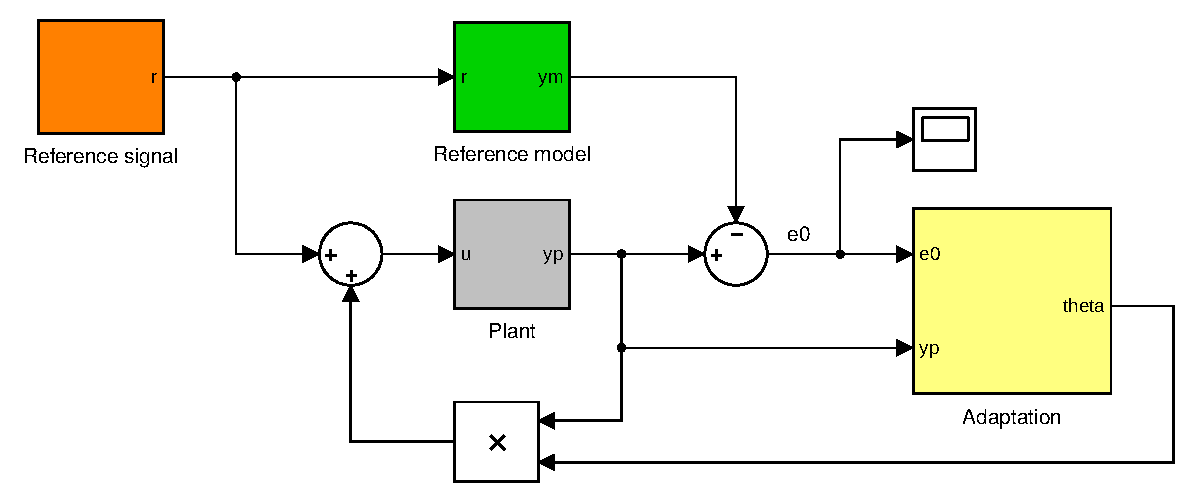
\includegraphics[width=14cm]{figs/MRAC-111.eps}
  \caption{Diagrama de blocos do sistema. \quad
  (Model: \HI{\texttt{MRAC-111.mdl}}) }
\end{figure}

%---------------------------------------------------------------------
\bigskip%
\begin{figure}[H]
  \centering
  \includegraphics[scale=0.8]{figs/plant.eps}
  \caption{Diagrama de blocos da planta.}
\end{figure}

%---------------------------------------------------------------------
\bigskip%
\begin{figure}[H]
  \centering
  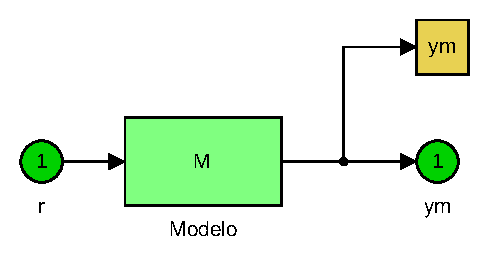
\includegraphics[scale=0.8]{figs/reference-model.eps}
  \caption{Diagrama de blocos do modelo de refer�ncia.}
\end{figure}

%---------------------------------------------------------------------
\bigskip%
\begin{figure}[H]
  \centering
  \includegraphics[scale=0.8]{figs/reference-signal.eps}
  \caption{Diagrama de blocos do gerador de sinais de refer�ncia.}
\end{figure}

%---------------------------------------------------------------------
\bigskip%
\begin{figure}[H]
  \centering
  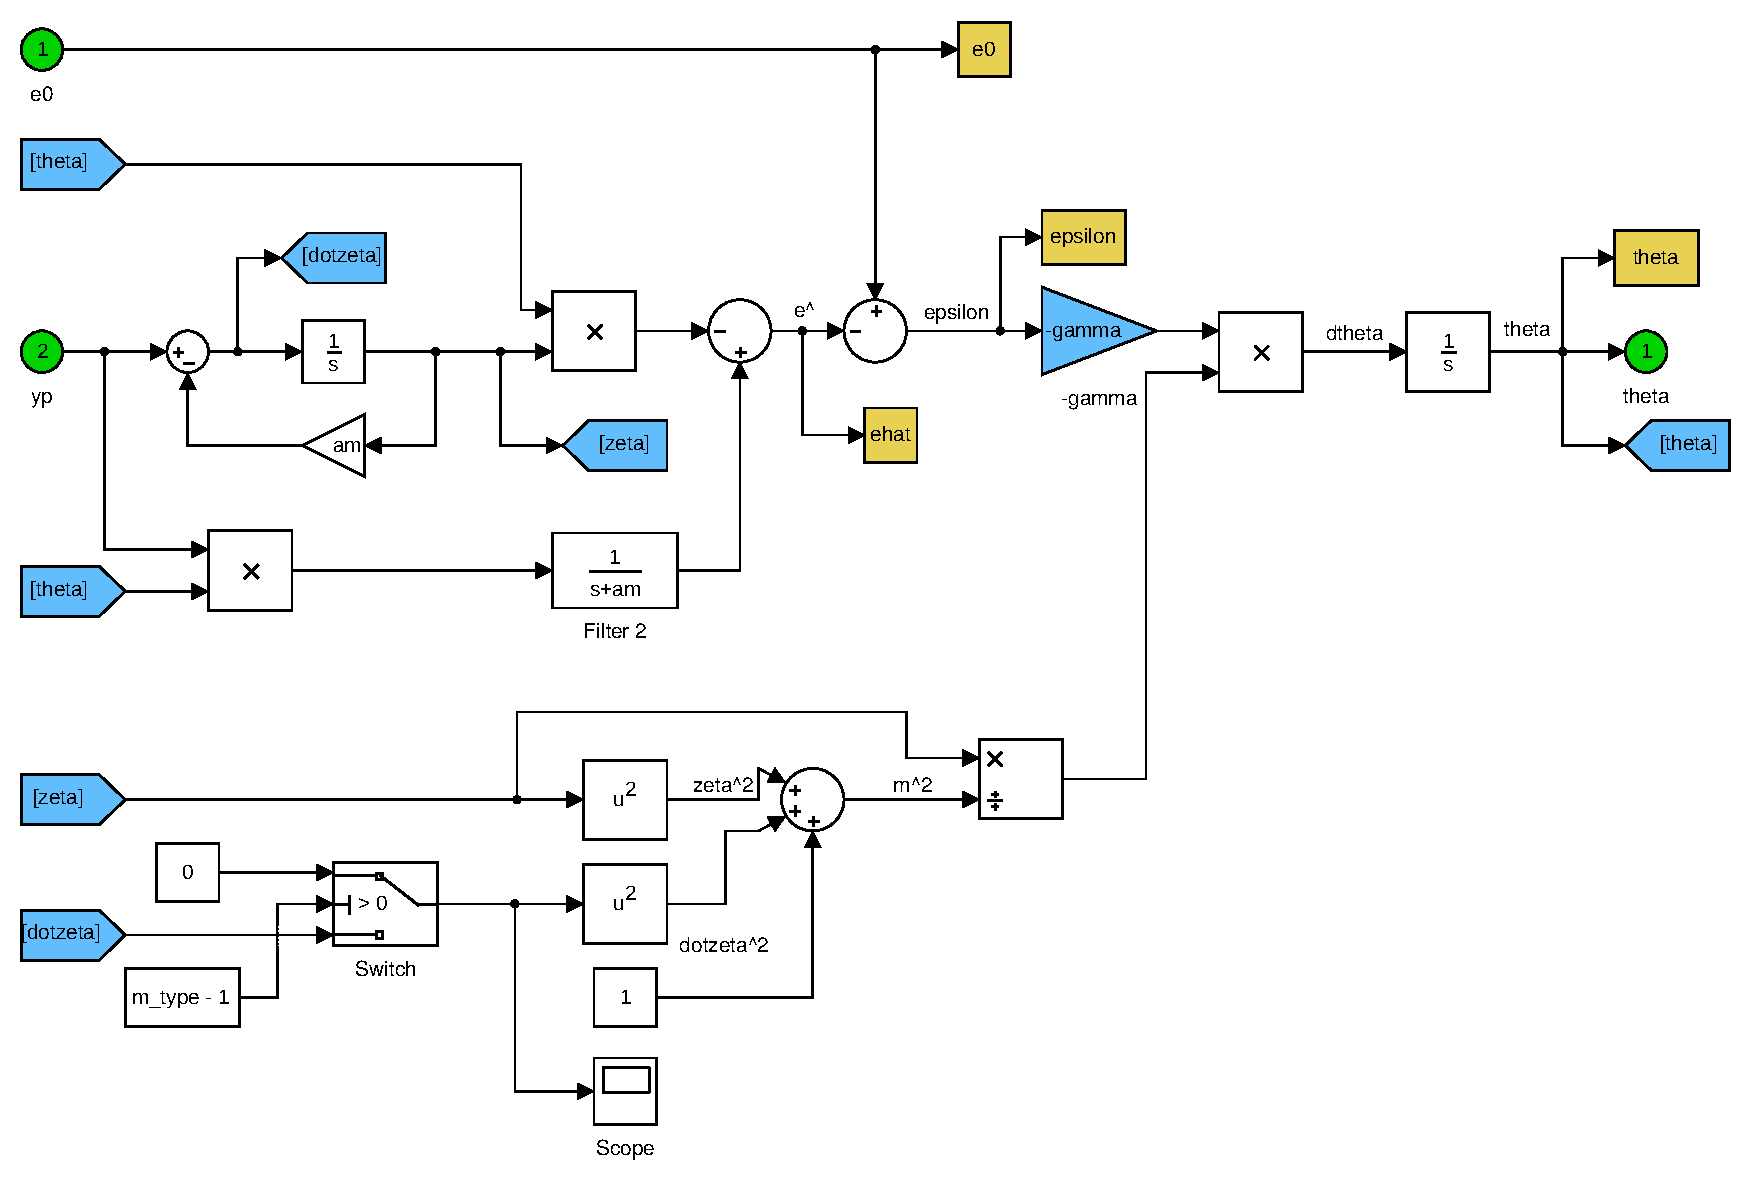
\includegraphics[width=16cm]{figs/adaptation.eps}
  \caption{Diagrama de blocos da lei de adapta��o.}
\end{figure}

\newpage%
%---------------------------------------------------------------------
\section{Resultados das simula��es}

Simula��o utilizando \HI{\texttt{Matlab/Simulink}}.

\subsection{Simula��o \#1}

\bigskip%
Par�metros e condi��es iniciais  :
%
\begin{align*}
  a_p &= -2\,,  &  y_p(0) &= 0\,, & \theta(0) &= 0\,, \\
  a_m &= 1\,,   &  y_m(0) &= 0\,, & \gamma &= 10,\ 100\,, \\
  r &= 1\,.
\end{align*}

\bigskip%
\begin{figure}[H]
  \centering
  \includegraphics[width=12cm]{figs/fig01d.eps} \\[2mm]
  \caption{Diagrama $e_0 \times \tilde{\theta}$.
  \hfill (Script: \HI{\tt simu01.m}) }
\end{figure}

\newpage%
%---------------------------------------------------------------------
\begin{figure}[H]
  \centering
  \includegraphics[width=12cm]{figs/fig01c.eps} \\[2mm]
  \includegraphics[width=12cm]{figs/fig01a.eps} \\[2mm]
  \includegraphics[width=12cm]{figs/fig01b.eps} \\[2mm]
  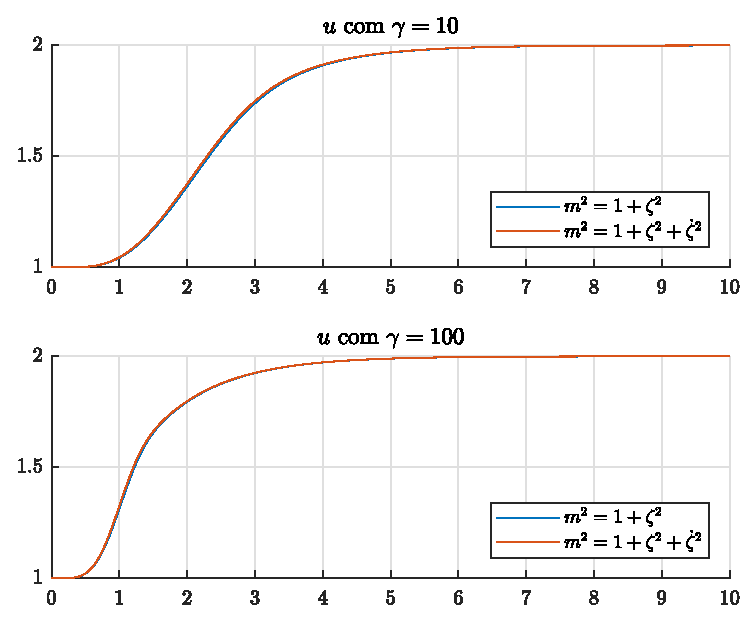
\includegraphics[width=12cm]{figs/fig01e.eps} \\[2mm]
  \caption{Resultado da simula��o com algoritmo Gradiente normalizado.
  \hfill (Script: \HI{\tt simu01.m}) }
\end{figure}


\newpage%
%---------------------------------------------------------------------
\subsection{Simula��o \#2}

\bigskip%
Par�metros e condi��es iniciais  :
%
\begin{align*}
  a_p &= -2\,,  &  y_p(0) &= \HI{2}\,, & \theta(0) &= 0\,, \\
  a_m &= 1\,,   &  y_m(0) &= 0\,, & \gamma &= 2,\ 100\,, \\
  r &= 1\,.
\end{align*}

\bigskip%
\begin{figure}[H]
  \centering
  \includegraphics[width=12cm]{figs/fig02d.eps} \\[2mm]
  \caption{Diagrama $e_0 \times \tilde{\theta}$.
  \hfill (Script: \HI{\tt simu02.m}) }
\end{figure}

\newpage%
%---------------------------------------------------------------------
\begin{figure}[H]
  \centering
  \includegraphics[width=12cm]{figs/fig02c.eps} \\[2mm]
  \includegraphics[width=12cm]{figs/fig02a.eps} \\[2mm]
  \includegraphics[width=12cm]{figs/fig02b.eps} \\[2mm]
  \includegraphics[width=12cm]{figs/fig02e.eps} \\[2mm]
  \caption{Resultado da simula��o com algoritmo Gradiente normalizado.
  \hfill (Script: \HI{\tt simu02.m}) }
\end{figure}

\newpage%
%---------------------------------------------------------------------
\subsection{Simula��o \#3}

\bigskip%
Par�metros e condi��es iniciais  :
%
\begin{align*}
  a_p &= -2\,,  &  y_p(0) &= \HI{10}\,, & \theta(0) &= 0\,, \\
  a_m &= 1\,,   &  y_m(0) &= 0\,, & \gamma &= 2,\ 100\,, \\
  r &= 1\,.
\end{align*}

\bigskip%
\begin{figure}[H]
  \centering
  \includegraphics[width=12cm]{figs/fig03d.eps} \\[2mm]
  \caption{Diagrama $e_0 \times \tilde{\theta}$.
  \hfill (Script: \HI{\tt simu03.m}) }
\end{figure}

\newpage%
%---------------------------------------------------------------------
\begin{figure}[H]
  \centering
  \includegraphics[width=12cm]{figs/fig03c.eps} \\[2mm]
  \includegraphics[width=12cm]{figs/fig03a.eps} \\[2mm]
  \includegraphics[width=12cm]{figs/fig03b.eps} \\[2mm]
  \includegraphics[width=12cm]{figs/fig03e.eps} \\[2mm]
  \caption{Resultado da simula��o com algoritmo Gradiente normalizado.
  \hfill (Script: \HI{\tt simu03.m}) }
\end{figure}


%---------------------------------------------------------------------
%\bibliographystyle{agsm}
%\bibliography{bib,coe736}

%---------------------------------------------------------------------
\end{document}
